\subsection{Damped Forced Vibrations ($b \neq 0$)}
\noindent
Our equation is 
\begin{equation*}
	my' + by' + ky = F_0\cos{(\gamma t)}.
\end{equation*}
Depending on if $\Delta = b^2 - 4mk$ is positive, zero, or negative, we'll get different results and thus different guesses for $y_p$ and thus different solutions.
There is, however, one long, complicated and not very useful for $y$.
\begin{equation*}
	y = C_1e^{\frac{-b+\sqrt{b^2-4mk}}{2m}t} + C_2e^{\frac{-b-\sqrt{b^2-4mk}}{2m}t} +
	 \frac{F_0\left(b\gamma\sin{(\gamma t)} + \left(k-\gamma^2m\right)\cos{(\gamma t)}\right)}{b^2\gamma^2 + (k-\gamma^2m)^2}.
\end{equation*}
The one useful thing this formula does tell us is that assuming $m$, $b$, $k$, $F_0$, and $\gamma$ are all positive and non-zero, the exponential terms quickly decrease to 0, so in the limit the function looks like the particular solution part.

\begin{center}
	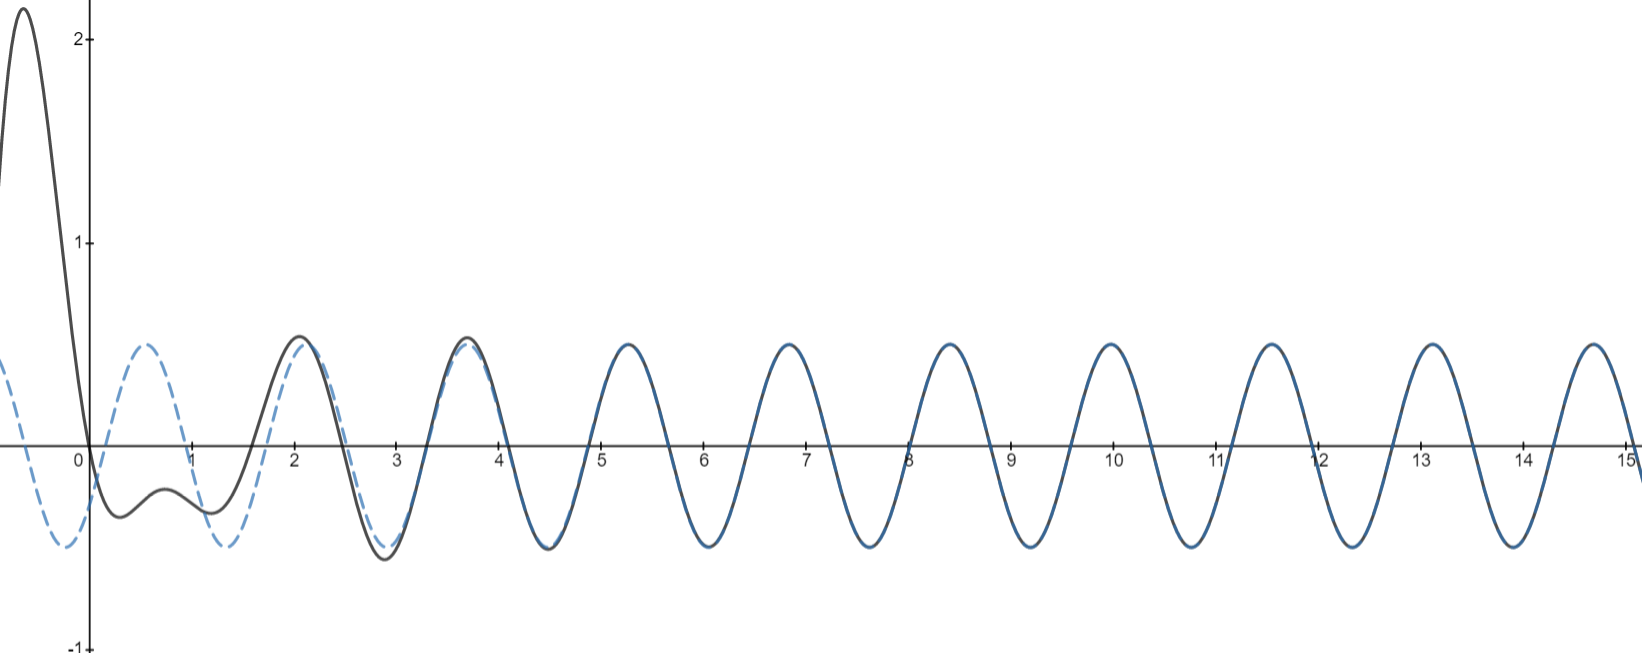
\includegraphics[width=0.75\textwidth]{./higherOrder/forcedVibrs/damped_forced.png}
\end{center}

\begin{example}
	Solve the following IVP.
	\begin{equation*}
		\begin{cases}
			y'' + 2y' + 10y = 5\cos{(4t)} \\
			y(0) = 0 \\
			y'(0) = -2.6
		\end{cases}
	\end{equation*}
\end{example}
\noindent
Some of the work has been omitted for brevity.

\noindent
Solving the auxiliary equation and finding $y_h$,
\begin{equation*}
	r^2 + 2r + 10 = 0 \implies r = -1 \pm 3i \implies y_h = e^{-t}\left(C_1\cos{(3t) + C_2\sin{(3t)}}\right).
\end{equation*}
Guessing the form of $y_p$, noting that $\omega \neq \gamma$,
\begin{equation*}
	y_p = A\cos{(4t)} + B\sin{(4t)}.
\end{equation*}
Solving for $A$ and $B$,
\begin{equation*}
	y_p'' + 2y_p' + 10y_p = 5\cos{(4t)} \implies A = -3/10 \text{ and } B = 4/10.
\end{equation*}
Solving for $C_1$ and $C_2$,
\begin{equation*}
	\begin{cases}
		y(0) = 0 \\
		y'(0) = -2.6
	\end{cases} \implies C_1 = 3/10 \text{ and } C_2 = -13/10.
\end{equation*}
So, we have a solution for $y$,
\begin{equation*}
	y = e^{-t}\left(\frac{3}{10}\cos{(3t)} - \frac{13}{10}\sin{(3t)}\right) + \left(\frac{-3}{10}\cos{(4t)} + \frac{4}{10}\sin{(4t)}\right).
\end{equation*}
The graph of this solution was shown above before the example.